\documentclass{../../note}

\usepackage{amsthm}
\usepackage{pgfplots}
\pgfplotsset{compat=1.18}
\newtheorem{example}{Example}
\usepackage{xcolor} % For colored text
\usepackage{tikz}
\usetikzlibrary{shapes,arrows,positioning,fit,calc,matrix}
\usepackage{algorithm}
\usepackage{algpseudocode}
\usepackage{listings}
\lstset{
  basicstyle=\ttfamily\small,
  keywordstyle=\color{blue},
  commentstyle=\color{green!60!black},
  stringstyle=\color{purple},
  numbers=left,
  numberstyle=\tiny,
  numbersep=5pt,
  breaklines=true,
  frame=single,
}

\title{数据结构 04}
\author{isomo}

\begin{document}

\maketitle

考纲内容:

\begin{itemize}

  \item \textbf{查找}\\
    查找的基本概念,线性表的查找,二叉排序树,哈希表的查找。

  \item \textbf{内排序}\\
    排序的基本概念,各种排序(插入排序、交换排序、选择排序、归并排序和基数排序)的基本思想和算法分析。
\end{itemize}

\section{查找}

\subsection{查找的基本概念}
\textcolor{red}{查找(Searching)}是在一个数据集合中寻找特定元素的过程。

\textbf{基本术语}:
\begin{itemize}
  \item \textcolor{red}{查找表(Search Table)}:由同一类型的数据元素组成的集合。
  \item \textcolor{red}{关键字(Key)}:数据元素中唯一标识该元素的属性。
  \item \textcolor{red}{查找长度(Search Length)}:查找过程中对比关键字的次数。
  \item \textcolor{red}{平均查找长度(Average Search Length, ASL)}:所有查找过程中对比关键字次数的期望值。
\end{itemize}

查找算法的性能评价依据主要为:
\begin{itemize}
  \item 平均查找长度(ASL)
  \item 时间复杂度
  \item 空间复杂度
\end{itemize}

\subsection{线性表的查找}

\subsubsection{顺序查找}
\textcolor{red}{顺序查找(Sequential Search)}是最基本的查找算法,适用于顺序表和链表等线性结构。

\begin{algorithm}
  \caption{顺序查找算法}
  \begin{algorithmic}[1]
    \Procedure{SequentialSearch}{$ST, key$}
    \State $i \gets 0$
    \While{$i < n$ \textbf{and} $ST[i].key \neq key$}
    \State $i \gets i + 1$
    \EndWhile
    \If{$i < n$}
    \Return $i$ \Comment{找到,返回位置}
    \Else
    \Return $-1$ \Comment{未找到,返回-1}
    \EndIf
    \EndProcedure
  \end{algorithmic}
\end{algorithm}

\colorbox{yellow}{顺序查找的平均时间复杂度为$O(n)$,最坏时间复杂度为$O(n)$。}

\subsubsection{折半查找}
\textcolor{red}{折半查找(Binary Search)}要求表中元素按关键字有序排列,且存储结构必须是随机存取的(如顺序表)。

\begin{algorithm}
  \caption{折半查找算法}
  \begin{algorithmic}[1]
    \Procedure{BinarySearch}{$ST, key, low, high$}
    \While{$low \leq high$}
    \State $mid \gets \lfloor (low + high) / 2 \rfloor$
    \If{$ST[mid].key = key$}
    \Return $mid$ \Comment{找到,返回位置}
    \ElsIf{$ST[mid].key > key$}
    \State $high \gets mid - 1$
    \Else
    \State $low \gets mid + 1$
    \EndIf
    \EndWhile
    \Return $-1$ \Comment{未找到,返回-1}
    \EndProcedure
  \end{algorithmic}
\end{algorithm}

\textcolor{blue}{折半查找的查找效率分析}:
\begin{itemize}
  \item 时间复杂度:$O(\log n)$
  \item 空间复杂度:$O(1)$
\end{itemize}

\colorbox{yellow}{折半查找比顺序查找效率高,但要求表必须有序且采用顺序存储结构。}

\subsubsection{分块查找}
\textcolor{red}{分块查找(Block Search)}介于顺序查找与折半查找之间,将表分为若干块,块内无序但块间有序。

步骤:
\begin{enumerate}
  \item 先在索引表中确定要查找的数据所在的块
  \item 然后在块内进行顺序查找
\end{enumerate}

\textcolor{blue}{分块查找的平均查找长度:}
\begin{align}
  ASL = \frac{s+1}{2} + \frac{b+1}{2}
\end{align}
其中,$s$为块数,$b$为每块的记录数。

\subsection{二叉排序树}

\textcolor{red}{二叉排序树(Binary Search Tree, BST)}是一种特殊的二叉树,满足以下条件:
\begin{itemize}
  \item 若左子树非空,则左子树上所有结点的值均小于根结点的值
  \item 若右子树非空,则右子树上所有结点的值均大于根结点的值
  \item 左右子树也分别是二叉排序树
\end{itemize}

\begin{figure}[h]
  \centering
  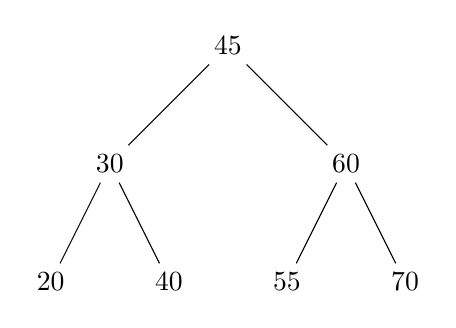
\begin{tikzpicture}[level distance=1.5cm,
      level 1/.style={sibling distance=3cm},
    level 2/.style={sibling distance=1.5cm}]
    \node {45}
    child {node {30}
      child {node {20}}
      child {node {40}}
    }
    child {node {60}
      child {node {55}}
      child {node {70}}
    };
  \end{tikzpicture}
  \caption{二叉排序树示例}
\end{figure}

\subsubsection{二叉排序树的基本操作}

\paragraph{查找操作}

\begin{algorithm}
  \caption{二叉排序树查找算法}
  \begin{algorithmic}[1]
    \Procedure{BSTSearch}{$T, key$}
    \If{$T = NULL$ \textbf{or} $key = T.data.key$}
    \Return $T$
    \ElsIf{$key < T.data.key$}
    \Return \Call{BSTSearch}{$T.lchild, key$}
    \Else
    \Return \Call{BSTSearch}{$T.rchild, key$}
    \EndIf
    \EndProcedure
  \end{algorithmic}
\end{algorithm}

\paragraph{插入操作}
在二叉排序树中插入一个结点,需保持其二叉排序树的性质。插入位置一定是某个叶结点的位置。

\paragraph{删除操作}
删除操作较为复杂,需考虑三种情况:
\begin{itemize}
  \item 删除叶结点:直接删除
  \item 删除只有一个子树的结点:用子树替代该结点
  \item 删除有两个子树的结点:用直接后继(中序遍历下的后继)替代,然后删除后继结点
\end{itemize}

二叉排序树的查找、插入和删除操作的平均时间复杂度均为$O(\log n)$,但最坏情况下会退化为$O(n)$(如树退化为单链表)。

\subsection{平衡二叉树}
\textcolor{red}{平衡二叉树(AVL树)}是一种特殊的二叉排序树,要求任一结点的左右子树高度差不超过1。

平衡因子BF(node) = 左子树高度 - 右子树高度,平衡二叉树中所有结点的平衡因子只能是-1、0或1。

插入结点后可能破坏平衡性,需通过旋转操作恢复:
\begin{itemize}
  \item LL型:单右旋
  \item RR型:单左旋
  \item LR型:先左后右双旋
  \item RL型:先右后左双旋
\end{itemize}

\textcolor{blue}{平衡二叉树的查找、插入和删除操作的时间复杂度均为$O(\log n)$。}

\subsection{哈希表的查找}

\textcolor{red}{哈希表(Hash Table)}是一种以"键-值"形式存储数据的数据结构,它通过哈希函数将关键字映射到表中的位置,实现高效查找。

\subsubsection{哈希函数}
常用的哈希函数构造方法:
\begin{itemize}
  \item 除留余数法:$h(key) = key \mod p$($p$通常选取小于表长的最大质数)
  \item 直接定址法:$h(key) = a \times key + b$
  \item 数字分析法:选取关键字的某些位作为哈希地址
  \item 平方取中法:取关键字平方后的中间几位作为哈希地址
\end{itemize}

\subsubsection{冲突处理}
\textcolor{red}{冲突(Collision)}指不同关键字映射到哈希表的同一位置。

\paragraph{开放定址法}
当发生冲突时,使用某种探测方法寻找下一个空位置:
\begin{itemize}
  \item 线性探测法:$h_i(key) = (h(key) + i) \mod m$
  \item 平方探测法:$h_i(key) = (h(key) + i^2) \mod m$
  \item 双散列法:$h_i(key) = (h(key) + i \times h_2(key)) \mod m$
\end{itemize}

\paragraph{链地址法}
将哈希表的每个位置设为链表的头节点,相同哈希地址的元素存储在同一链表中。

\begin{figure}[h]
  \centering
  \begin{tikzpicture}
    \matrix (m) [matrix of nodes, row sep=0.3cm, column sep=0.8cm] {
      0 & $\rightarrow$ & 10 & $\rightarrow$ & 20 \\
      1 & $\rightarrow$ & 31 & & \\
      2 & $\rightarrow$ & 12 & $\rightarrow$ & 22 & $\rightarrow$ & 32 \\
      3 & & & & \\
      4 & $\rightarrow$ & 34 & & \\
    };
    \draw[thick] (m-1-1.north west) -- (m-1-1.north east) -- (m-5-1.south east) -- (m-5-1.south west) -- cycle;
  \end{tikzpicture}
  \caption{链地址法示例}
\end{figure}

\subsubsection{哈希表性能分析}

\textcolor{blue}{装填因子(Load Factor)}:$\alpha = \frac{n}{m}$,其中$n$是表中记录数,$m$是哈希表长度。

装填因子衡量哈希表的满度,它直接影响查找效率。一般$\alpha \leq 0.75$时查找效率较高。

\colorbox{yellow}{哈希表的查找效率:}
\begin{itemize}
  \item 最好情况:$O(1)$,没有冲突直接定位
  \item 最坏情况:$O(n)$,全部冲突退化为线性查找
  \item 平均情况:取决于哈希函数和冲突处理方法,通常近似为$O(1)$
\end{itemize}

哈希表的优点是查找、插入、删除操作的时间复杂度接近$O(1)$,但缺点是需要额外的存储空间,且无法实现有序操作。

\section{内排序}

\subsection{排序的基本概念}

\textcolor{red}{排序(Sorting)}是将一组数据按照特定的顺序进行重新排列的过程。

\textbf{基本术语}:
\begin{itemize}
  \item \textcolor{red}{内排序}:排序过程中数据元素全部存放在内存中进行的排序
  \item \textcolor{red}{外排序}:排序过程中需要在内外存间多次交换数据的排序
  \item \textcolor{red}{稳定性}:若两个记录$R_i$和$R_j$的关键字相同且排序前$R_i$在$R_j$之前,排序后$R_i$仍在$R_j$之前,则称排序算法是稳定的
\end{itemize}

\textbf{排序算法的评价指标}:
\begin{itemize}
  \item 时间复杂度:比较次数和移动次数
  \item 空间复杂度:执行算法所需的额外存储空间
  \item 算法的稳定性:关键字相同的记录是否保持原有的相对位置
\end{itemize}

\colorbox{yellow}{常见排序算法的时间复杂度比较:}
\begin{center}
  \begin{tabular}{|c|c|c|c|c|c|}
    \hline
    \textbf{算法} & \textbf{平均时间} & \textbf{最好情况} & \textbf{最坏情况} & \textbf{空间复杂度} & \textbf{稳定性} \\
    \hline
    直接插入排序 & $O(n^2)$ & $O(n)$ & $O(n^2)$ & $O(1)$ & 稳定 \\
    \hline
    希尔排序 & $O(n^{1.3})$ & $O(n)$ & $O(n^2)$ & $O(1)$ & 不稳定 \\
    \hline
    冒泡排序 & $O(n^2)$ & $O(n)$ & $O(n^2)$ & $O(1)$ & 稳定 \\
    \hline
    快速排序 & $O(n\log{n})$ & $O(n\log{n})$ & $O(n^2)$ & $O(\log{n})$ & 不稳定 \\
    \hline
    简单选择排序 & $O(n^2)$ & $O(n^2)$ & $O(n^2)$ & $O(1)$ & 不稳定 \\
    \hline
    堆排序 & $O(n\log{n})$ & $O(n\log{n})$ & $O(n\log{n})$ & $O(1)$ & 不稳定 \\
    \hline
    归并排序 & $O(n\log{n})$ & $O(n\log{n})$ & $O(n\log{n})$ & $O(n)$ & 稳定 \\
    \hline
    基数排序 & $O(d(n+r))$ & $O(d(n+r))$ & $O(d(n+r))$ & $O(r)$ & 稳定 \\
    \hline
  \end{tabular}
\end{center}
其中,$n$为待排序记录数,$d$为关键字位数,$r$为关键字取值范围。

\subsection{插入排序}

\subsubsection{直接插入排序}
\textcolor{red}{直接插入排序(Straight Insertion Sort)}的基本思想是将一个记录插入到已经排好序的有序表中,得到一个新的、记录数增加1的有序表。

\begin{algorithm}
  \caption{直接插入排序算法}
  \begin{algorithmic}[1]
    \Procedure{InsertionSort}{$A[0...n-1]$}
    \For{$i \gets 1$ to $n-1$}
    \State $temp \gets A[i]$ \Comment{保存当前元素}
    \State $j \gets i - 1$ \Comment{前一位置}
    \While{$j \geq 0$ \textbf{and} $A[j] > temp$}
    \State $A[j+1] \gets A[j]$ \Comment{元素后移}
    \State $j \gets j - 1$
    \EndWhile
    \State $A[j+1] \gets temp$ \Comment{插入到正确位置}
    \EndFor
    \EndProcedure
  \end{algorithmic}
\end{algorithm}

\begin{figure}[h]
  \centering
  \begin{tikzpicture}
    \matrix (m) [matrix of nodes, nodes={draw, minimum width=0.8cm, minimum height=0.8cm}, row sep=0.2cm] {
      49 & 38 & 65 & 97 & 76 & 13 & 27 & 49 \\
    };

    \node[right=0.5cm of m-1-8] (step1) {初始数组};

    \matrix (m2) [below=0.5cm of m, matrix of nodes, nodes={draw, minimum width=0.8cm, minimum height=0.8cm}, row sep=0.2cm] {
      \textcolor{red}{38} & 49 & 65 & 97 & 76 & 13 & 27 & 49 \\
    };

    \node[right=0.5cm of m2-1-8] (step2) {第1次插入后};

    \matrix (m3) [below=0.5cm of m2, matrix of nodes, nodes={draw, minimum width=0.8cm, minimum height=0.8cm}, row sep=0.2cm] {
      \textcolor{red}{13} & 27 & 38 & 49 & 49 & 65 & 76 & 97 \\
    };

    \node[right=0.5cm of m3-1-8] (step3) {最终排序结果};

  \end{tikzpicture}
  \caption{直接插入排序示例}
\end{figure}

\textcolor{blue}{直接插入排序的性能分析}:
\begin{itemize}
  \item 时间复杂度:平均$O(n^2)$,最好$O(n)$,最坏$O(n^2)$
  \item 空间复杂度:$O(1)$
  \item 稳定性:稳定
\end{itemize}

\colorbox{yellow}{直接插入排序适用于基本有序的数据集合或者数据集合较小的情况。}

\subsubsection{希尔排序}
\textcolor{red}{希尔排序(Shell Sort)}是插入排序的一种改进版本,也称为"缩小增量排序"。其基本思想是将整个待排记录序列分割成若干子序列分别进行直接插入排序。

\begin{algorithm}
  \caption{希尔排序算法}
  \begin{algorithmic}[1]
    \Procedure{ShellSort}{$A[0...n-1]$}
    \State 选择一个增量序列$d_1, d_2, ..., d_t$,其中$d_t=1$
    \For{$k \gets 1$ to $t$}
    \State 按增量$d_k$对各子序列进行直接插入排序
    \EndFor
    \EndProcedure
  \end{algorithmic}
\end{algorithm}

\textcolor{blue}{希尔排序的性能分析}:
\begin{itemize}
  \item 时间复杂度:取决于增量序列,一般为$O(n^{1.3})$
  \item 空间复杂度:$O(1)$
  \item 稳定性:不稳定
\end{itemize}

\subsection{交换排序}

\subsubsection{冒泡排序}
\textcolor{red}{冒泡排序(Bubble Sort)}的基本思想是通过相邻元素的比较和交换,使较大的元素逐渐"浮"到后面。

\begin{algorithm}
  \caption{冒泡排序算法}
  \begin{algorithmic}[1]
    \Procedure{BubbleSort}{$A[0...n-1]$}
    \For{$i \gets 0$ to $n-2$}
    \State $swapped \gets false$
    \For{$j \gets 0$ to $n-2-i$}
    \If{$A[j] > A[j+1]$}
    \State 交换$A[j]$和$A[j+1]$
    \State $swapped \gets true$
    \EndIf
    \EndFor
    \If{$swapped = false$}
    \State \Return \Comment{数组已经有序,提前结束}
    \EndIf
    \EndFor
    \EndProcedure
  \end{algorithmic}
\end{algorithm}

\textcolor{blue}{冒泡排序的性能分析}:
\begin{itemize}
  \item 时间复杂度:平均$O(n^2)$,最好$O(n)$,最坏$O(n^2)$
  \item 空间复杂度:$O(1)$
  \item 稳定性:稳定
\end{itemize}

\subsubsection{快速排序}
\textcolor{red}{快速排序(Quick Sort)}的基本思想是通过一趟排序将待排记录分隔成独立的两部分,其中一部分记录的关键字均比另一部分的关键字小,然后再分别对这两部分记录继续进行排序。

\begin{algorithm}
  \caption{快速排序算法}
  \begin{algorithmic}[1]
    \Procedure{QuickSort}{$A, low, high$}
    \If{$low < high$}
    \State $pivot \gets$ \Call{Partition}{$A, low, high$}
    \State \Call{QuickSort}{$A, low, pivot-1$}
    \State \Call{QuickSort}{$A, pivot+1, high$}
    \EndIf
    \EndProcedure
    \State
    \Procedure{Partition}{$A, low, high$}
    \State $pivot \gets A[low]$ \Comment{选择第一个元素作为基准}
    \While{$low < high$}
    \While{$low < high$ \textbf{and} $A[high] \geq pivot$}
    \State $high \gets high - 1$
    \EndWhile
    \State $A[low] \gets A[high]$
    \While{$low < high$ \textbf{and} $A[low] \leq pivot$}
    \State $low \gets low + 1$
    \EndWhile
    \State $A[high] \gets A[low]$
    \EndWhile
    \State $A[low] \gets pivot$
    \Return $low$
    \EndProcedure
  \end{algorithmic}
\end{algorithm}

\textcolor{blue}{快速排序的性能分析}:
\begin{itemize}
  \item 时间复杂度:平均$O(n\log{n})$,最好$O(n\log{n})$,最坏$O(n^2)$
  \item 空间复杂度:$O(\log{n})$
  \item 稳定性:不稳定
\end{itemize}

\colorbox{yellow}{快速排序是实践中最高效的排序算法之一,但在最坏情况下性能会显著下降。}

\subsection{选择排序}

\subsubsection{简单选择排序}
\textcolor{red}{简单选择排序(Simple Selection Sort)}的基本思想是每一趟从待排序的数据元素中选出最小(或最大)的一个元素,顺序放在已排好序的数列的最后,直到全部待排序的数据元素排完。

\begin{algorithm}
  \caption{简单选择排序算法}
  \begin{algorithmic}[1]
    \Procedure{SelectionSort}{$A[0...n-1]$}
    \For{$i \gets 0$ to $n-2$}
    \State $min \gets i$
    \For{$j \gets i+1$ to $n-1$}
    \If{$A[j] < A[min]$}
    \State $min \gets j$
    \EndIf
    \EndFor
    \If{$min \neq i$}
    \State 交换$A[i]$和$A[min]$
    \EndIf
    \EndFor
    \EndProcedure
  \end{algorithmic}
\end{algorithm}

\textcolor{blue}{简单选择排序的性能分析}:
\begin{itemize}
  \item 时间复杂度:平均$O(n^2)$,最好$O(n^2)$,最坏$O(n^2)$
  \item 空间复杂度:$O(1)$
  \item 稳定性:不稳定
\end{itemize}

\subsubsection{堆排序}
\textcolor{red}{堆排序(Heap Sort)}是利用堆这种数据结构所设计的一种排序算法。

\textcolor{red}{堆(Heap)}是具有以下性质的完全二叉树:每个节点的值都大于或等于其左右孩子节点的值(大顶堆);或者每个节点的值都小于或等于其左右孩子节点的值(小顶堆)。

\begin{algorithm}
  \caption{堆排序算法}
  \begin{algorithmic}[1]
    \Procedure{HeapSort}{$A[0...n-1]$}
    \For{$i \gets \lfloor n/2 \rfloor - 1$ downto $0$} \Comment{建堆}
    \State \Call{Heapify}{$A, n, i$}
    \EndFor
    \For{$i \gets n-1$ downto $1$} \Comment{堆排序}
    \State 交换$A[0]$和$A[i]$ \Comment{将堆顶元素与末尾元素交换}
    \State \Call{Heapify}{$A, i, 0$} \Comment{重新调整堆}
    \EndFor
    \EndProcedure
    \State
    \Procedure{Heapify}{$A, n, i$} \Comment{调整以i为根的子树}
    \State $largest \gets i$
    \State $left \gets 2 \times i + 1$
    \State $right \gets 2 \times i + 2$
    \If{$left < n$ \textbf{and} $A[left] > A[largest]$}
    \State $largest \gets left$
    \EndIf
    \If{$right < n$ \textbf{and} $A[right] > A[largest]$}
    \State $largest \gets right$
    \EndIf
    \If{$largest \neq i$}
    \State 交换$A[i]$和$A[largest]$
    \State \Call{Heapify}{$A, n, largest$}
    \EndIf
    \EndProcedure
  \end{algorithmic}
\end{algorithm}

\begin{figure}[h]
  \centering
  \begin{tikzpicture}[level distance=1.2cm,
      level 1/.style={sibling distance=3cm},
    level 2/.style={sibling distance=1.5cm}]
    \node {4}
    child {node {10}
      child {node {14}}
      child {node {19}}
    }
    child {node {9}
      child {node {16}}
      child {node {18}}
    };
  \end{tikzpicture}
  \quad
  $\Rightarrow$
  \quad
  \begin{tikzpicture}[level distance=1.2cm,
      level 1/.style={sibling distance=3cm},
    level 2/.style={sibling distance=1.5cm}]
    \node {19}
    child {node {18}
      child {node {14}}
      child {node {4}}
    }
    child {node {16}
      child {node {10}}
      child {node {9}}
    };
  \end{tikzpicture}
  \caption{从无序数组构建大顶堆的示例}
\end{figure}

\textcolor{blue}{堆排序的性能分析}:
\begin{itemize}
  \item 时间复杂度:平均$O(n\log{n})$,最好$O(n\log{n})$,最坏$O(n\log{n})$
  \item 空间复杂度:$O(1)$
  \item 稳定性:不稳定
\end{itemize}

\colorbox{yellow}{堆排序是选择排序的一种优化,具有比简单选择排序更好的时间复杂度。}

\subsection{归并排序}

\textcolor{red}{归并排序(Merge Sort)}是采用分治法的一个典型应用。其基本思想是将两个或两个以上的有序表合并成一个新的有序表。

\begin{algorithm}
  \caption{归并排序算法}
  \begin{algorithmic}[1]
    \Procedure{MergeSort}{$A, left, right$}
    \If{$left < right$}
    \State $mid \gets \lfloor (left + right) / 2 \rfloor$
    \State \Call{MergeSort}{$A, left, mid$}
    \State \Call{MergeSort}{$A, mid+1, right$}
    \State \Call{Merge}{$A, left, mid, right$}
    \EndIf
    \EndProcedure
    \State
    \Procedure{Merge}{$A, left, mid, right$}
    \State 创建临时数组$temp[left...right]$
    \State $i \gets left$, $j \gets mid+1$, $k \gets left$
    \While{$i \leq mid$ \textbf{and} $j \leq right$}
    \If{$A[i] \leq A[j]$}
    \State $temp[k] \gets A[i]$
    \State $i \gets i + 1$, $k \gets k + 1$
    \Else
    \State $temp[k] \gets A[j]$
    \State $j \gets j + 1$, $k \gets k + 1$
    \EndIf
    \EndWhile
    \While{$i \leq mid$} \Comment{处理剩余元素}
    \State $temp[k] \gets A[i]$
    \State $i \gets i + 1$, $k \gets k + 1$
    \EndWhile
    \While{$j \leq right$} \Comment{处理剩余元素}
    \State $temp[k] \gets A[j]$
    \State $j \gets j + 1$, $k \gets k + 1$
    \EndWhile
    \For{$k \gets left$ to $right$} \Comment{将临时数组复制回原数组}
    \State $A[k] \gets temp[k]$
    \EndFor
    \EndProcedure
  \end{algorithmic}
\end{algorithm}

\begin{figure}[h]
  \centering
  \begin{tikzpicture}[
      level 1/.style={sibling distance=40mm},
      level 2/.style={sibling distance=20mm},
      level 3/.style={sibling distance=10mm},
    ]
    \node {38,27,43,3,9,82,10}
    child {node {38,27,43,3}
      child {node {38,27}
        child {node {38}}
        child {node {27}}
      }
      child {node {43,3}
        child {node {43}}
        child {node {3}}
      }
    }
    child {node {9,82,10}
      child {node {9}
      }
      child {node {82,10}
        child {node {82}}
        child {node {10}}
      }
    };

    \draw[->] (0,-3.8) -- (0,-4.2) node[midway, right] {合并};

    \matrix (m1) [below=4.5cm of m-1-1, matrix of nodes, nodes={draw, minimum width=0.7cm, minimum height=0.7cm}] {
      27 & 38 & 3 & 43 & 9 & 10 & 82 \\
    };

    \draw[->] (0,-4.8) -- (0,-5.2) node[midway, right] {最终合并};

    \matrix (m2) [below=5.5cm of m-1-1, matrix of nodes, nodes={draw, minimum width=0.7cm, minimum height=0.7cm}] {
      3 & 9 & 10 & 27 & 38 & 43 & 82 \\
    };
  \end{tikzpicture}
  \caption{归并排序示例}
\end{figure}

\textcolor{blue}{归并排序的性能分析}:
\begin{itemize}
  \item 时间复杂度:平均$O(n\log{n})$,最好$O(n\log{n})$,最坏$O(n\log{n})$
  \item 空间复杂度:$O(n)$
  \item 稳定性:稳定
\end{itemize}

\colorbox{yellow}{归并排序是稳定的排序方法,并且具有稳定的时间复杂度,但需要额外的空间。}

\subsection{基数排序}

\textcolor{red}{基数排序(Radix Sort)}是一种非比较型排序算法,它根据关键字中的位值,将待排序的元素分配到桶中,达到排序的目的。

\begin{algorithm}
  \caption{基数排序算法(LSD,从低位到高位)}
  \begin{algorithmic}[1]
    \Procedure{RadixSort}{$A[0...n-1], d$} \Comment{d为最大位数}
    \For{$i \gets 1$ to $d$} \Comment{从最低位开始}
    \State 按第$i$位数字将所有元素分配到桶$bucket[0...9]$中
    \State 将所有桶中的元素依次收集到数组$A$中
    \EndFor
    \EndProcedure
  \end{algorithmic}
\end{algorithm}

\begin{figure}[h]
  \centering
  \begin{tikzpicture}[
      bucket/.style={draw, rectangle, minimum width=2cm, minimum height=0.8cm}
    ]
    \node[above] at (0,0) {原始数据: 329, 457, 657, 839, 436, 720, 355};

    \node[above] at (-3,-1) {按个位排序:};
    \node[bucket] at (0,-1.5) {720};
    \node[bucket] at (0,-2.3) {355};
    \node[bucket] at (0,-3.1) {436};
    \node[bucket] at (0,-3.9) {457};
    \node[bucket] at (0,-4.7) {657};
    \node[bucket] at (0,-5.5) {329};
    \node[bucket] at (0,-6.3) {839};

    \draw[->] (1.5,-3) -- (2.5,-3);

    \node[above] at (4,-1) {结果: 720, 355, 436, 457, 657, 329, 839};

    \node[above] at (4,-4) {继续按十位排序...};
  \end{tikzpicture}
  \caption{基数排序示例(按个位排序的第一步)}
\end{figure}

\textcolor{blue}{基数排序的性能分析}:
\begin{itemize}
  \item 时间复杂度:$O(d(n+r))$,其中$d$是关键字位数,$r$是关键字范围(桶的个数)
  \item 空间复杂度:$O(n+r)$
  \item 稳定性:稳定
\end{itemize}

\colorbox{yellow}{基数排序不进行关键字之间的比较,适用于数据量大但是每个数据位数不是很多的情况。}

\subsection{排序算法选择}

在实际应用中,选择合适的排序算法需要考虑以下因素:

\begin{itemize}
  \item \textbf{数据规模}:对于小规模数据,简单的排序算法如插入排序可能更高效;对于大规模数据,复杂度为$O(n\log{n})$的排序算法更合适
  \item \textbf{数据分布}:对于接近有序的数据,插入排序和冒泡排序可能表现更好
  \item \textbf{稳定性要求}:如果需要保持相同关键字元素的相对位置,应选择稳定的排序算法
  \item \textbf{存储要求}:如果内存空间有限,应避免使用需要额外空间的算法
  \item \textbf{关键字的性质}:对于整数或者可以转化为整数的关键字,可以考虑使用桶排序或基数排序
\end{itemize}

在实践中,许多编程语言的标准库采用混合策略,例如对小规模数据使用插入排序,对大规模数据使用快速排序或归并排序。

\end{document}